\chapter{Literature Review} \label{Chp: LiteratureReview}

In this chapter, we will start by introducing the building components of WSN, mainly focuses on different protocol options at each layer. Then we move to security related work, in three aspects of traffic analysis attacks against different Internet applications, attacks against certain protocols and methods for detecting information leakage in different scenarios. Finally we conclude the chapter by cross referencing those  attacks on Internet to the observable metadata in WSN, proposing the potential traffic features that may lead to information leakage.

In network terminology, 8 bits is called an OCTET. For the purpose of readability we use the general computer science term BYTE to represent the unit consists of 8 bits.

\section{Building Blocks of WSN}
In this section we categorise the components of WSN by OSI model\cite{OSI}.

The OSI model is a classic model in describing the communication between computing systems (\Cref{fig: OSI model}). The data channel is constructed layer by layer, from the physical medium at the bottom to the abstracted application at the top. Each layer serves a specific purpose, from how to transmit a bit between two physically connected devices to how applications interprets the data.

Before the application data is being sent over the wire, two ends of the communication must agree on protocols being used at each layer. The data is then encapsulated from top layer down to the bottom, as depicted in \Cref{fig: OSI channel}. Each encapsulation adds additional metadata, namely protocol headers, to the data. The process is unwound at the receiving side. Normally lower layer protocols are transparent to upper layers.The outputted encapsulated data from upper layer is simply treated as the payload to a lower layer protocol.

In many cases the boundaries between top three layers are ambiguous; thus they are all referred as Application Layer for convenience.

\begin{figure*}
	\centering
	{
		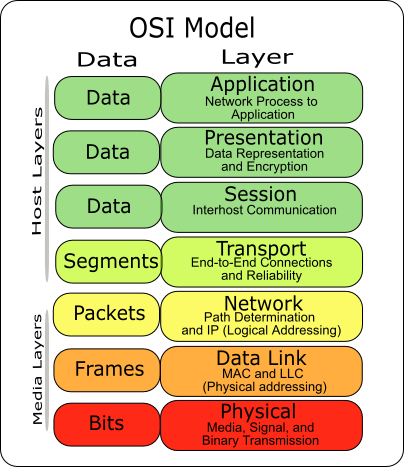
\includegraphics[width=0.4\textwidth,]{fig/Osi-model-jb.png}
	}
	\caption{OSI model} \label{fig: OSI model}
\end{figure*}

\begin{figure*}
	\centering
	{
		\includegraphics[width=0.6\textwidth,]{fig/Osi-model.png}
	}
	\caption{Data Transfer in OSI model} \label{fig: OSI channel}
\end{figure*}

\subsection{Physical Layer}
Physical Layer specifies the hardware requirements for devices. It defines data transmission at bit level.

WSN features, as explained by its name, wireless connectivity. 802.15.4\cite{802154} standard is supported in many recent WSN devices. Its Physical Layer specification is intended to be for embedded devices emphasising low energy, low cost and low speed. Bluetooth Low Energy, BLE, is another candidate for WSN with similar features. \cite{802154BLE} provides a performance analysis of 802.15.4 and BLE.

\subsection{Data Link Layer} \label{Subsec: Data Link Layer}
Data Link Layer solves the problem of how the media is controlled. It also defines the atomic data chunk, called frames, being transmitted over the physical channel. Data Link protocols are strongly related to physical features of underlining devices. This layer is sometimes referred as MAC layer and the frame is called MAC frame in many context. MAC protocol only solves single hop communication. Packet forward is defined in upper layer protocols.

With respect to Media Access Control, MAC, technologies such as CSMA/CA \cite{802154} standard and TSCH\cite{TSCH} provides solutions to at which timing and channel should the radio transceiver send and receive data. ContikiMAC\cite{ContikiMAC} proposes a Radio Duty Cycle, RDC, protocol that aims to be energy efficient and has been implemented on Contiki OS.

Another major component in Data Link Layer protocols is the format of different types of frames. In this research, We focus on 802.15.4 standard as its increasing attention in both industry and academy. There are four types of frames defined in this standard, which are:
\begin{description}
	\item[\textbf{Beacon}] broadcastes to physically organise the network.
	\item[\textbf{Command}] is used in network maintenance.
	\item[\textbf{Data}] carries actual payload.
	\item[\textbf{ACK}] only optionally sent in response when requested.
\end{description}

Among these types of frames, we are particularly interested in Data frames. We will explain our concern of this choice later in \Cref{Sec: Leakage Sources}. \Cref{Tbl: 802154 frame} describes the format of a 802.15.4 Data frame.

\begin{table*}[h!]
	\centering
		\begin{tabular}{|c|c|c|c|c|}
		\hline
		\multicolumn{3}{|c|}{MAC Header}                           & MAC Payload & MAC Footer     \\ \hline
		2 (bytes)     & 1                    & 4 to 20              & *           & 2              \\ \hline
		Frame Control & Data Sequence Number & Address Information & Data        & Frame Checksum \\ \hline
		\end{tabular}
	\caption{802.15.4 Data Frame}
	\label{Tbl: 802154 frame}
\end{table*}

We briefly explain the format of 802.15.4 Data frame.
\begin{description}[style=nextline]
	\item[\textbf{Frame Control}]
	This 2 bytes field contains the bit flags of additional information that instructs how the receiver should interpret this frame, including the type of this frame, whether the security option is enabled and how the source and destination addresses are represented. When the security option is enabled, additional field will be added to the frame. We will explain the security enabled frame format later in \Cref{Subsec: Data Link Layer}. A full explanation of the flags can be found in \cite{802154}.
	
	\item[\textbf{Sequence Number}]
	Each packet is assigned a sequence number. The main purpose of this field is that it enables a simple acknowledgement mechanism, ACK, at MAC layer. Since MAC layer provides only unreliable transmission, i.e. MAC frames are allowed to be dropped or arrive disordered; hence the ACK is optional. However, some other protocol can utilise this ACK, e.g. ContikiMAC uses the ACK MAC frame to inform the sender that the frame is received and hence terminates the resending process of sender.
	
	\item[\textbf{Address Information}]
	This field contains the source address and destination address of this frame. The length of address is variable. Simply speaking, a longer addresses is used for larger network. and shorter for smaller. Each device has a unique built in address as known as MAC address. The MAC address is configurable on some, in fact nearly all recently, devices. Broadcast is achieved by using a specific destination address but group multicast is not implemented on this layer. In fact, given the physical character of radio, both broadcast messages and unicast messages are technically broadcasted. It entirely depends on the receiver to dropping frames that specifies an unicast address of other nodes.
	
	\item[\textbf{Data}]
	This is the MAC layer data. This data is constituted of upper layer protocol headers and application data.
	
	\item[\textbf{Frame Checksum}]
	The checksum is used to check and correct the error induced by physical channel.
\end{description}

The Frame Control, Sequence Number and Address Information together are called MAC header. The Data field is called MAC payload accordingly. 802.15.4 standard specifies the Maximum Transmission Unit, MTU, to be 128 bytes.

Setting the security flag in Frame Control enables 802.15.4 security and adds additional information into the MAC header. We introduce the 802.15.4 security later in \Cref{Subsubsec: 802154 Sec}.

\subsubsection{802.15.4 Security} \label{Subsubsec: 802154 Sec}
802.15.4 security is an Authenticated Encryption with Associated Data, AEAD, scheme. To be more specifically, it provides encryption for MAC payload and authenticity for both MAC header and MAC payload. The cryptographic primitive adopts AES-128 as the block cipher.

802.15.4 has a set of configurable security levels:
\begin{itemize}
\item Encryption only, i.e. only MAC payload is encrypted in CTR mode.
\item Authentication only, i.e. a tag is attached at the end of Data field. The tag is computed on MAC header and MAC payload in CBC mode. The MAC payload is transmitted in plaintext.
\item Encryption and authentication. The whole frame is processed in CCM*\cite{802154} mode, with MAC header being the associated data and MAC payload being the plaintext to be encrypted. The asterisk symbol represents a slight restriction which requires the nonce, or IV, must contain the encoded format specifier that can uniquely determine the format of output ciphertext. In other words, the receiver must can uniquely determine by the nonce whether authentication and encryption are enabled as well as the length of authentication tag.
\item The authentication tag can be further configured to be 32 bit, 64 bit or 128 bit when it is enabled.
\end{itemize}

Figure.

CCM* for AEAD. AES-CBC MAC for auth. AES-CTR for enc.

ACL.

\subsection{Network Layer}

\subsection{Transport Layer}

\subsection{Application Layer}

%\cite{802154Sec} discusses some security concerns in 802.15.4.  LLSEC\cite{LLSEC} is the implementation of 802.15.4 security in Contiki.
%
%tinydtls\cite{tinydtls} is the implementation of DTLS we used in DTLS related experiments.
%
%To our knowledge, this is the first work of application fingerprinting through traffic analysis over wireless sensor network.

\section{Security Related Work}

\section{Potential Leakage Sources} \label{Sec: Leakage Sources}
%Why only look at MAC Data Frames